%\section{Scénario d'utilisation}
\chapter{Scénario d'utilisation}
\markboth{\MakeUppercase{Scénario d'utilisation}}{}     

	\section{Aspect général}

		%\centerline{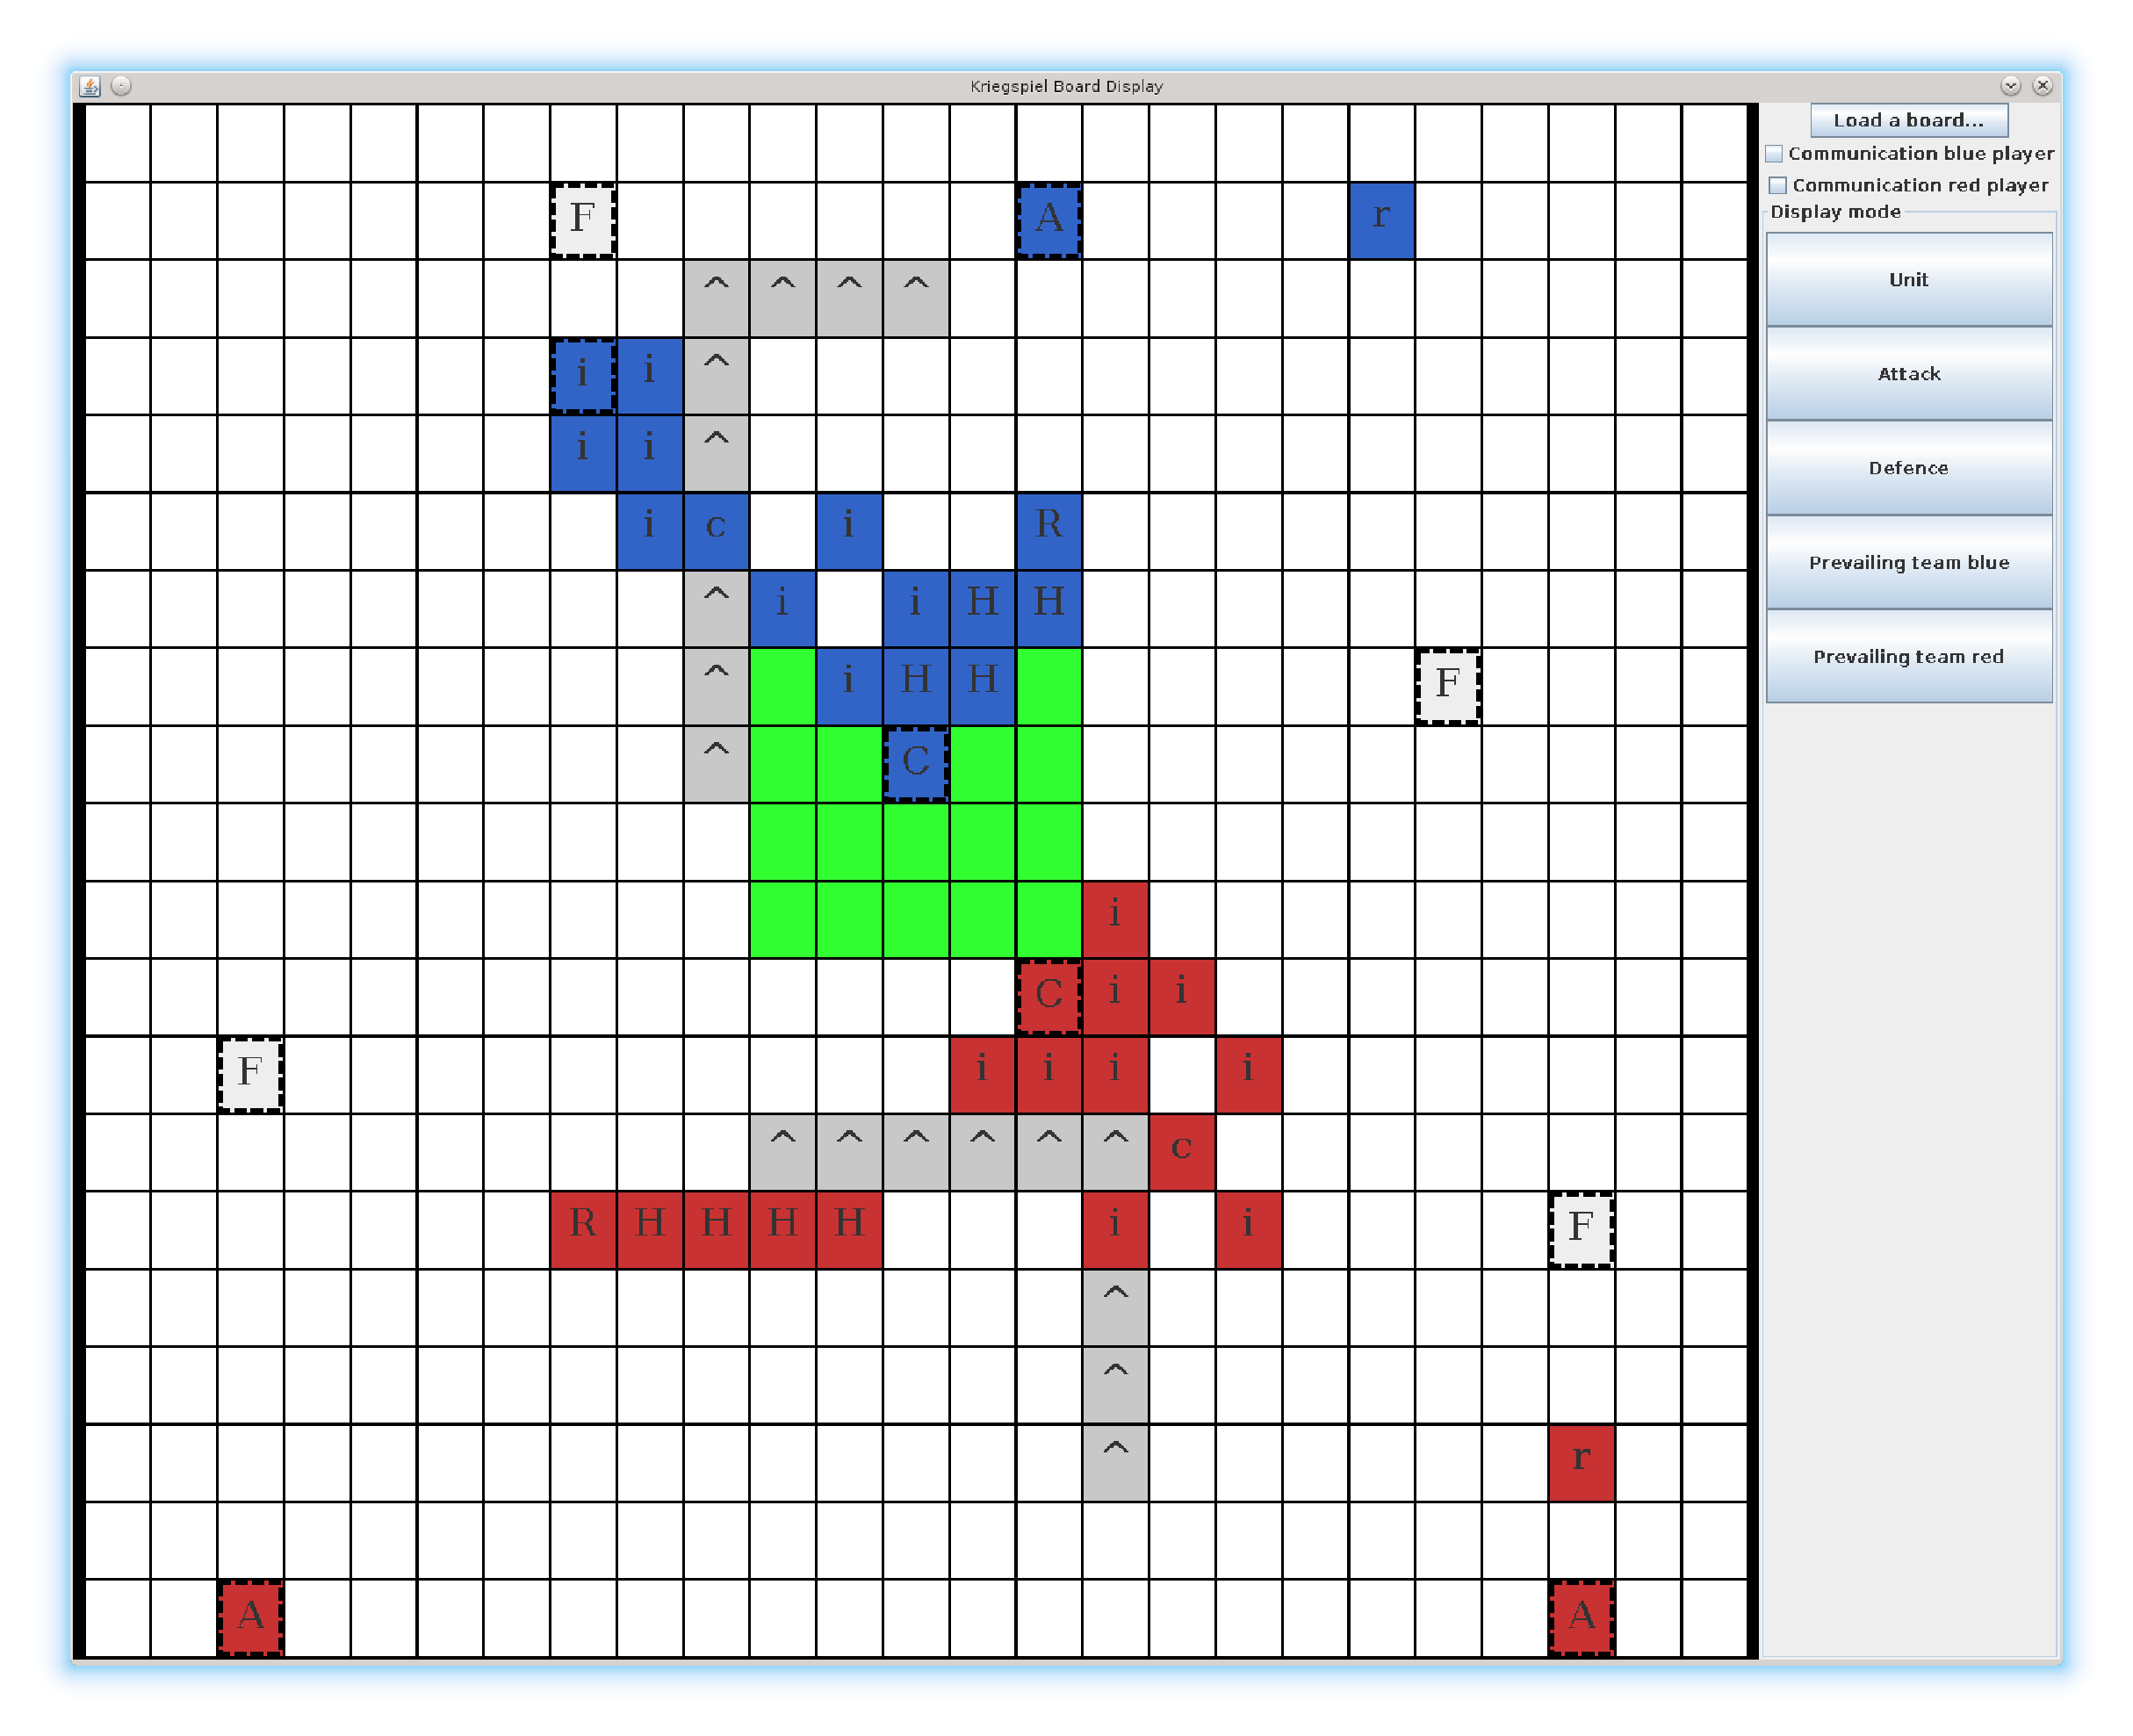
\includegraphics[scale=0.45]{images/screen1.eps}}

		\paragraph{Le plateau :}
			L'affichage du plateau prend la majorité de la fenêtre.
			Les entités sont représentées par des lettres dans des cases de la couleur de leur équipe.
			Les \^{} sur fond gris sont les montagnes.
			Les cases possédant une bordure pointillée noire sont les entités qui peuvent contenir une autre entité	(les arsenaux et les forts).
			Les cases vertes représentent les possibilités de mouvement	de l'entité sélectionnée (ici le SwiftCanon bleu). 
			Notons que l'unité ne peut pas se déplacer sur une case déja occupée.
			Lorsqu'une entité risque d'être détruite au prochain tour, son symbole est entouré de ( ).
			Lorsqu'elle est forcée de se retirer au prochain tour, son symbole est entouré de [ ].
	
		\paragraph{Le menu :}
	
			Le menu contient différents éléments :
			\begin{itemize}
			\item[-]Le bouton de chargement en haut permet de charger une situation depuis un fichier
			\item[-]Les checkboxes permettent d'activer ou de désactiver les communications
			\item[-]Les grands boutons permettent de changer le mode d'affichage
			\end{itemize}

	\section{Les modes d'affichage}

		\subsection{Mode unités}

			\centerline{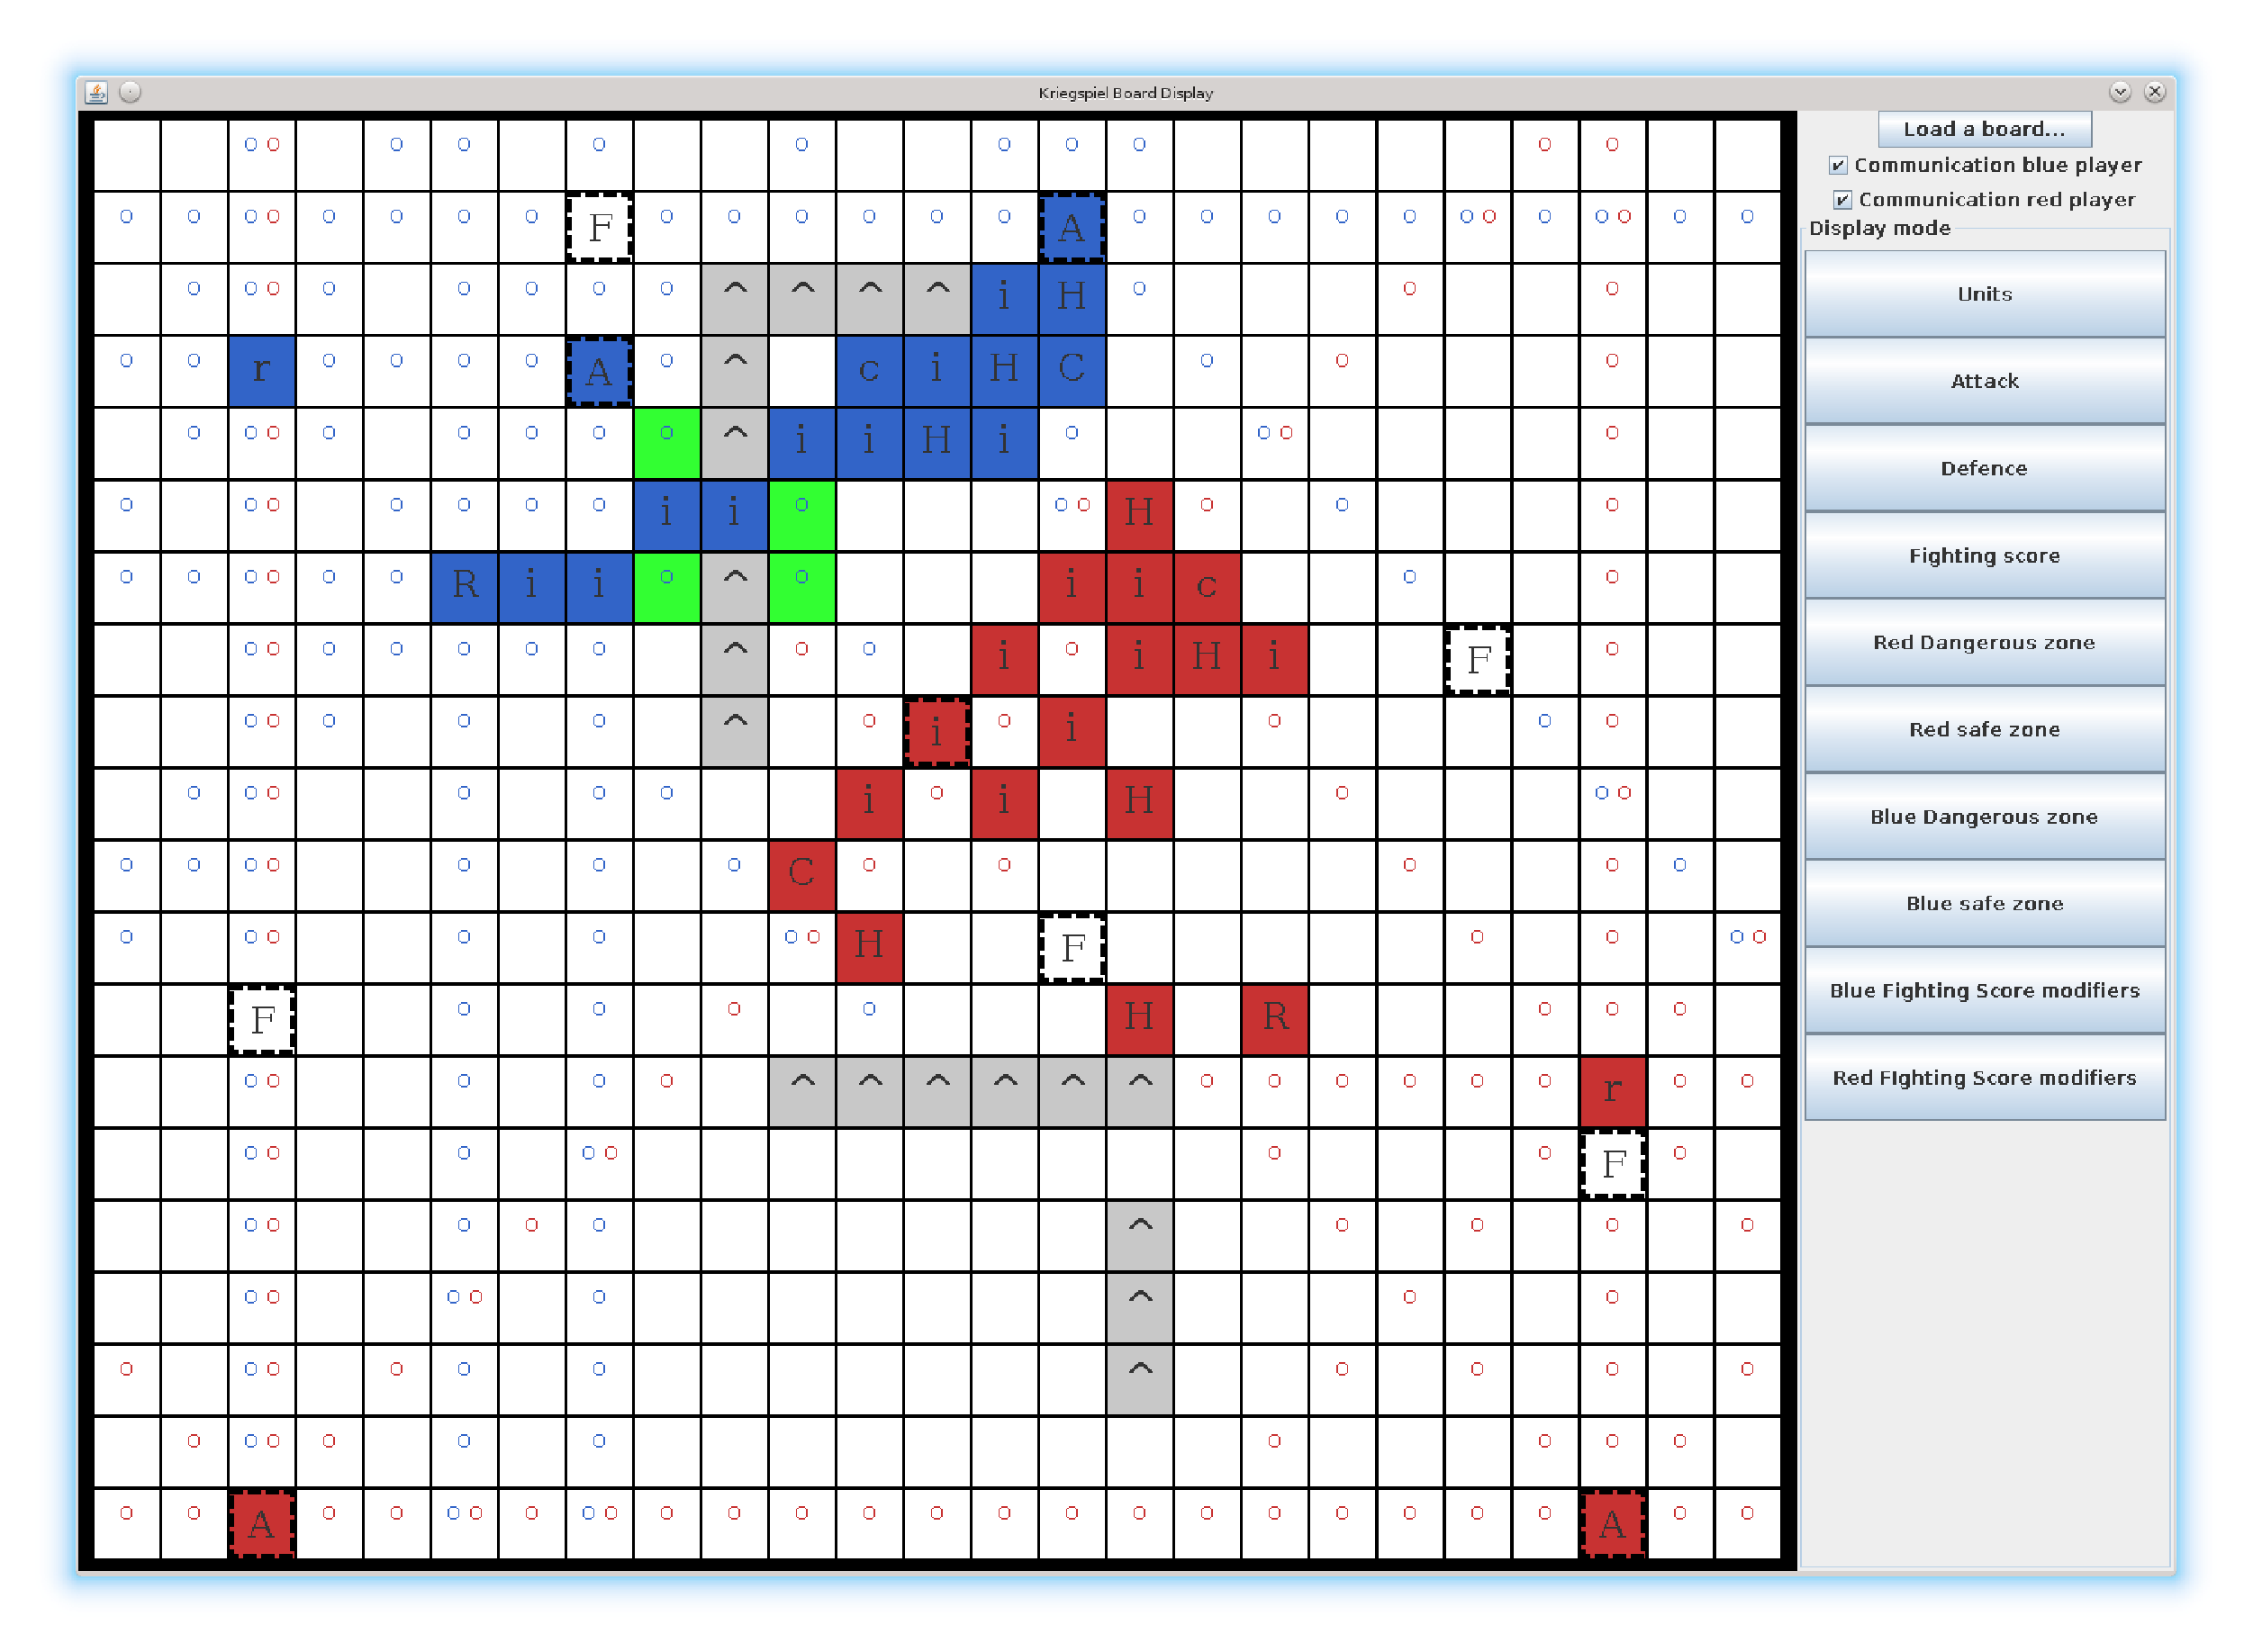
\includegraphics[scale=0.5]{images/screen_units.eps}}
			C'est le mode d'affichage principal, les symboles des unités sont affichés dans les cases.

			\clearpage

		\subsection{Modes attaque/défense}

			\centerline{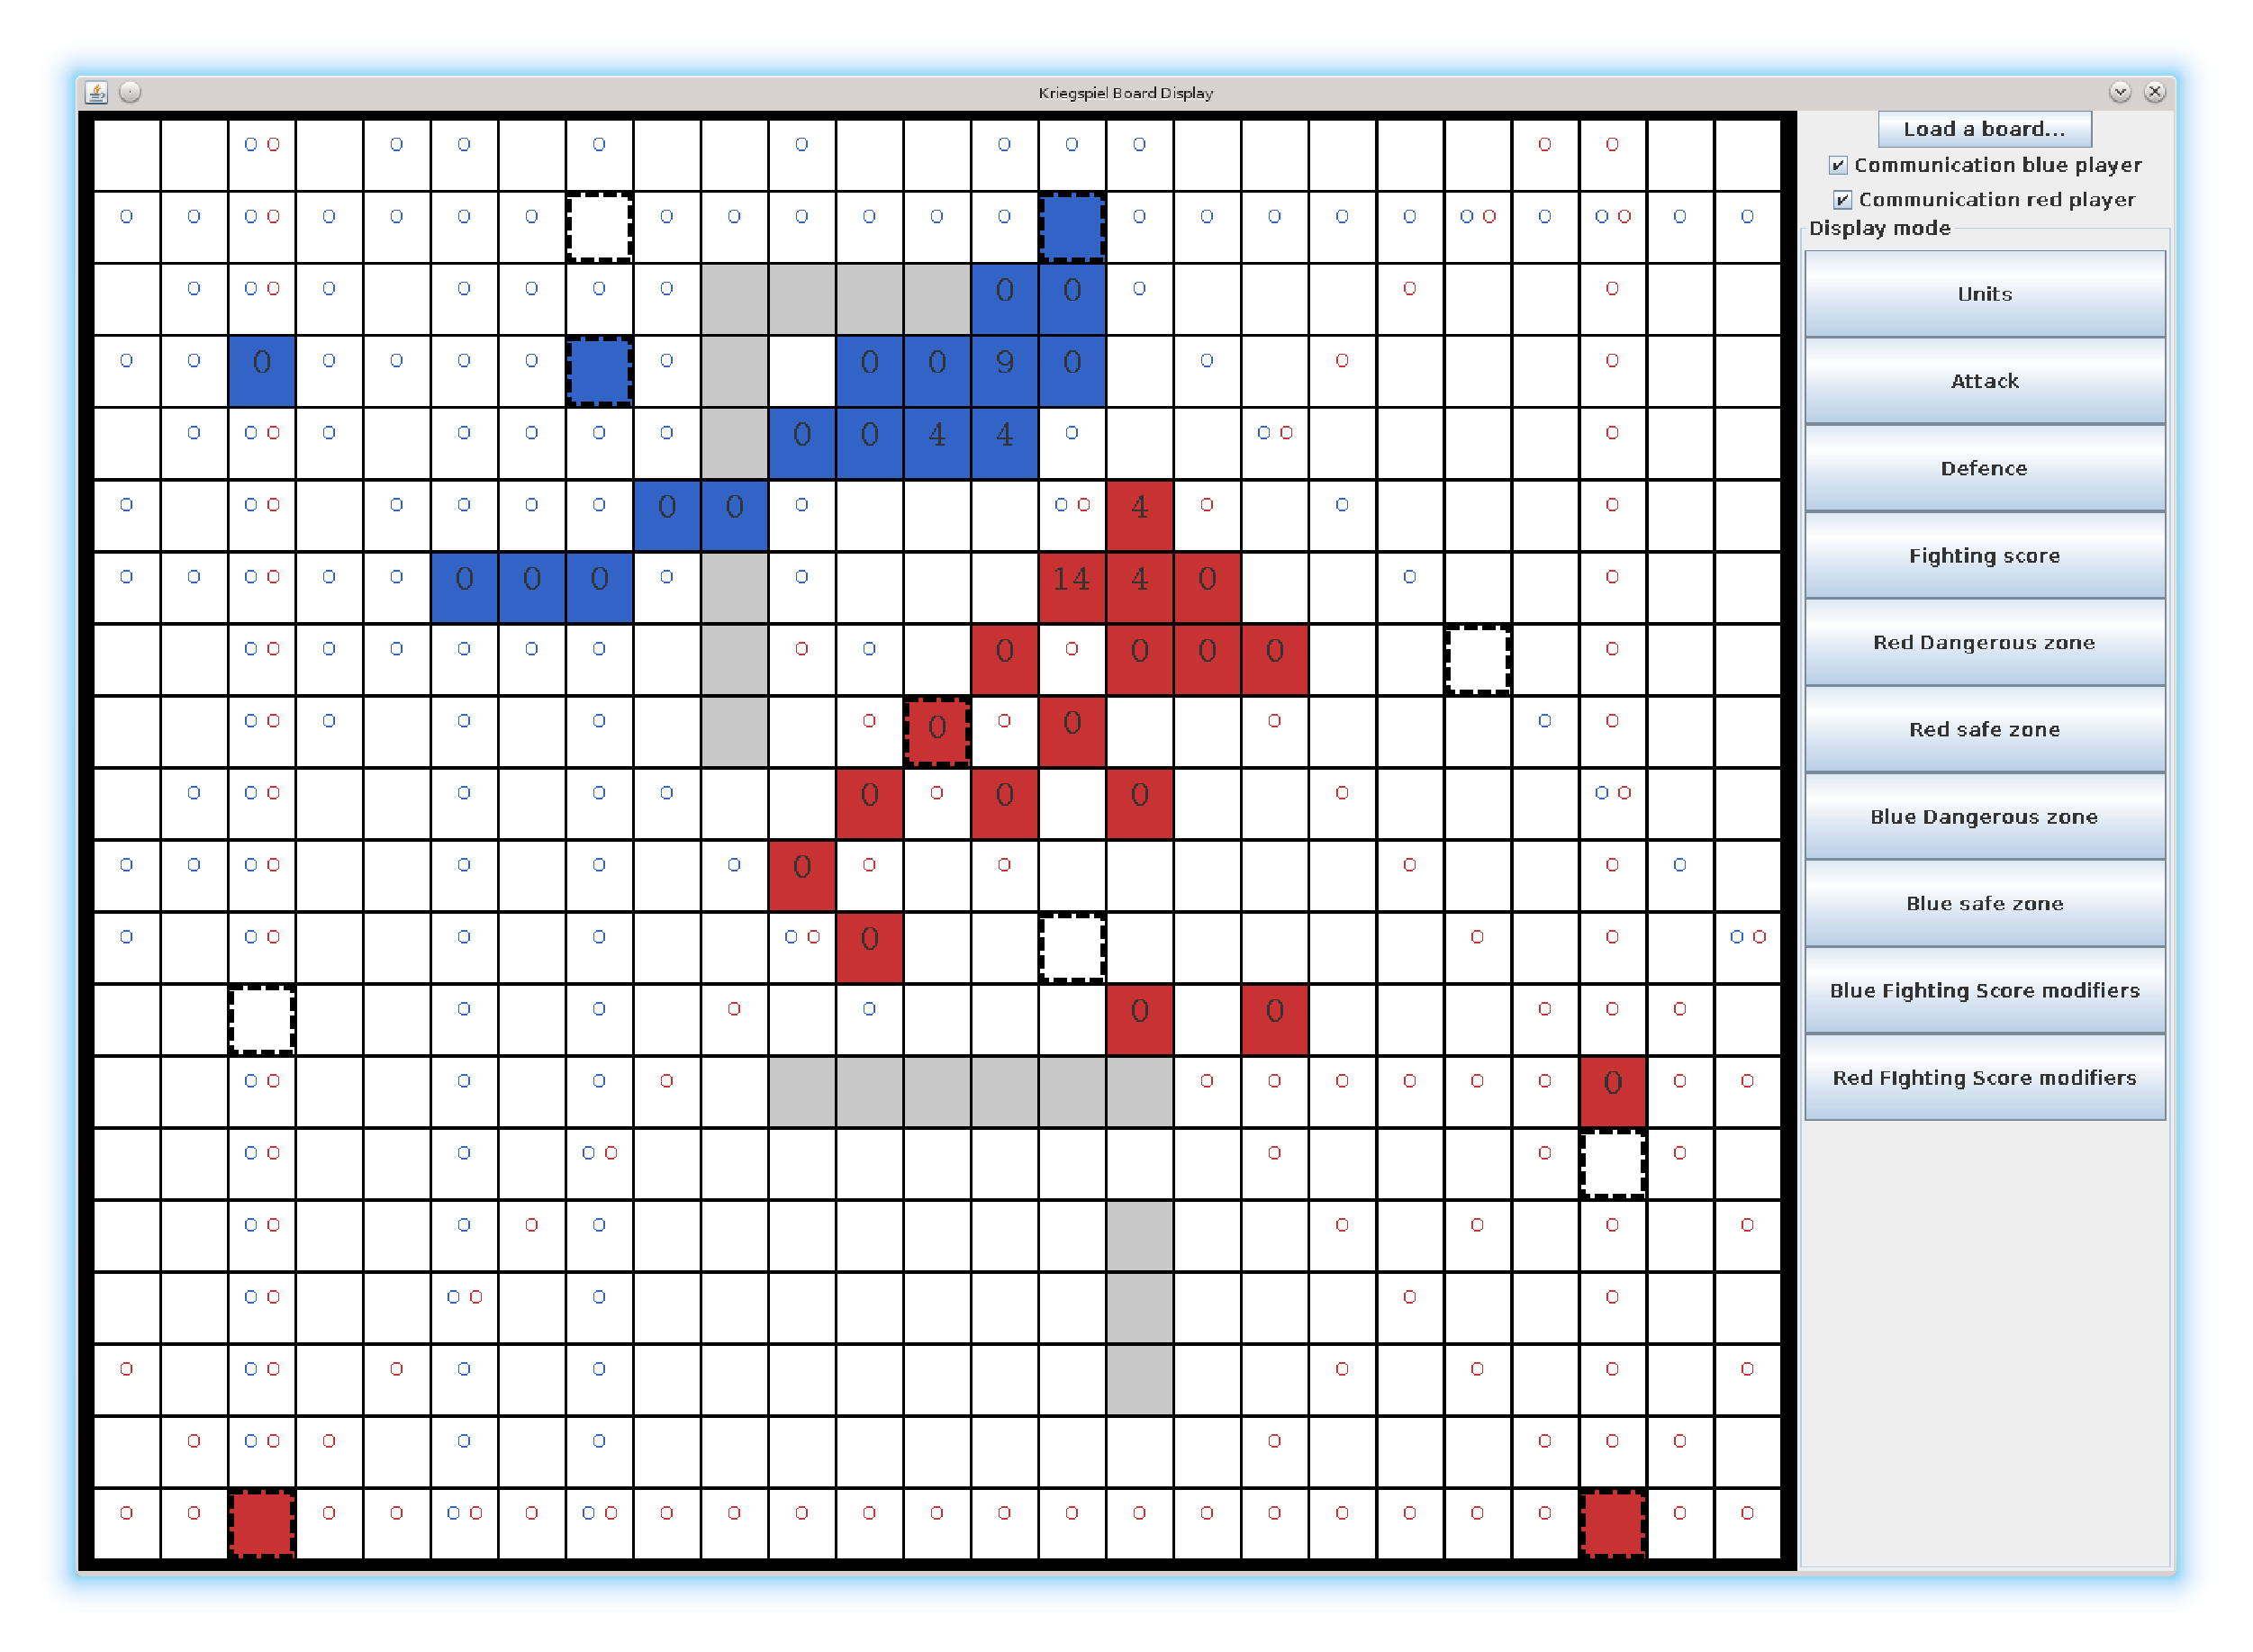
\includegraphics[scale=0.5]{images/screen_def.eps}}
			Dans le mode attaque, le total d'attaque potentielle subie est affiché à la place du symbole de chaque unité.
			Dans le mode défense, le total de défense de l'unité est affiché.
		
			\clearpage	

		\subsection{Mode score de combat}

			\centerline{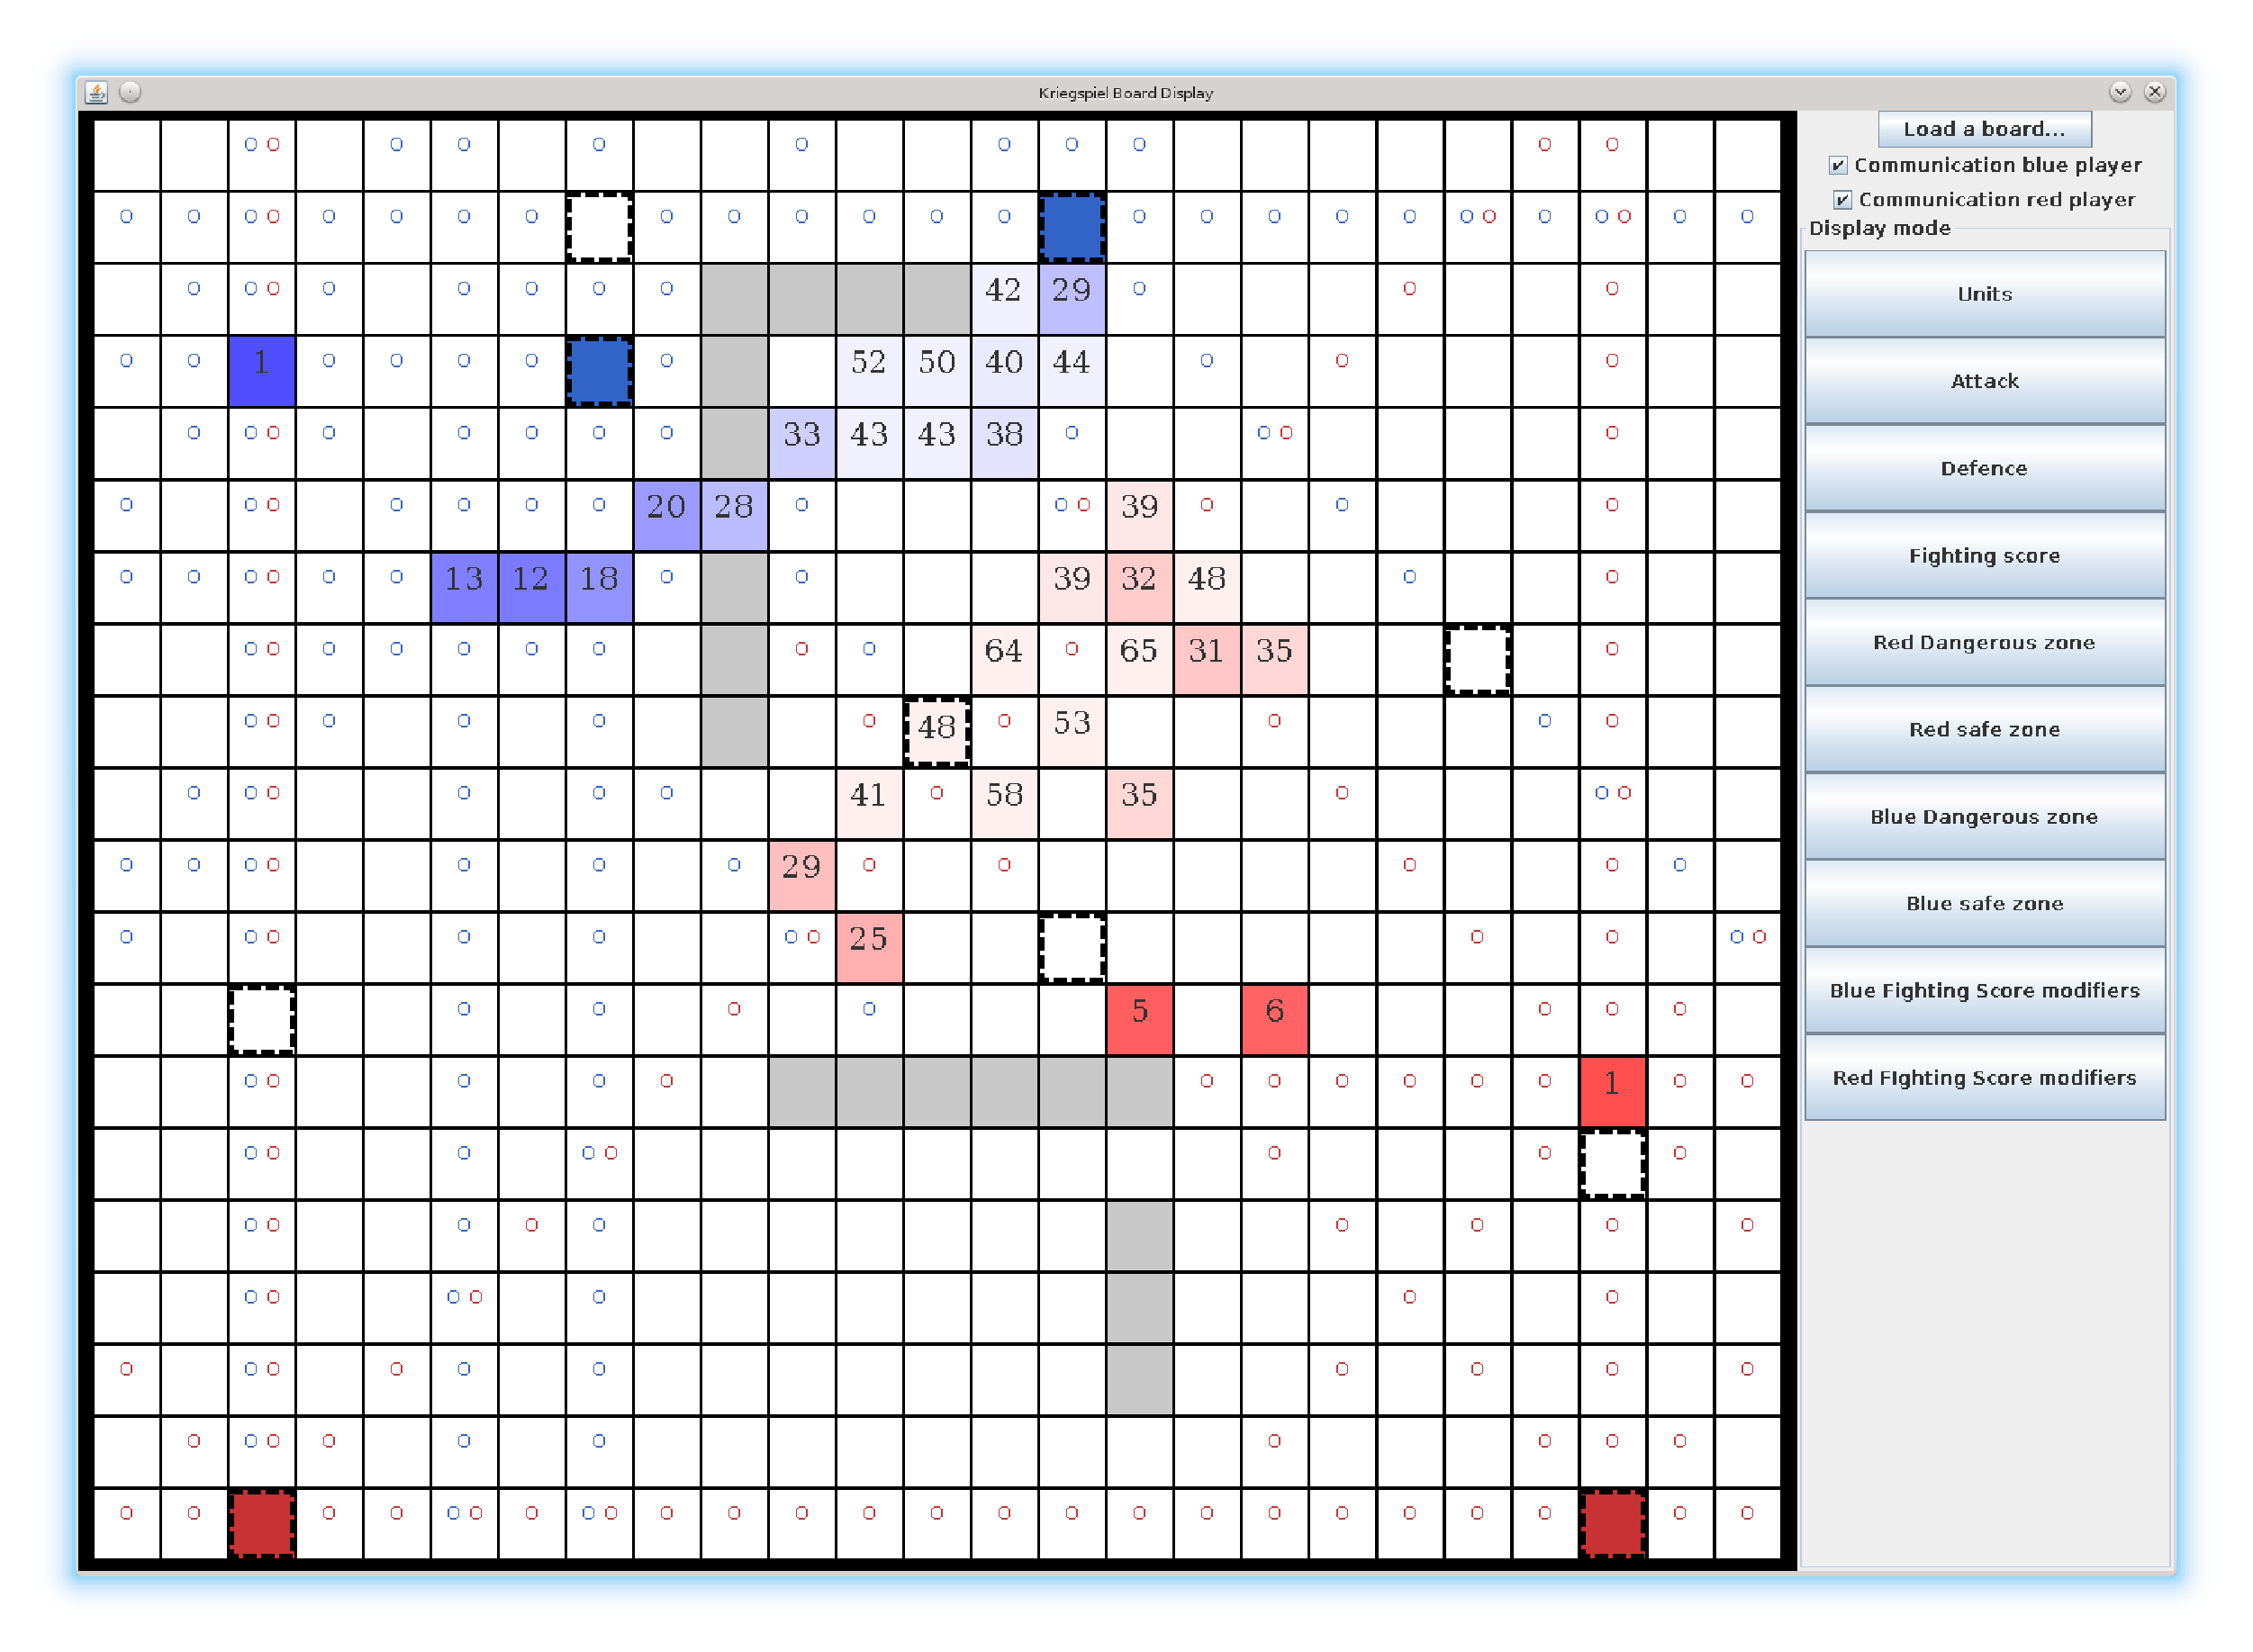
\includegraphics[scale=0.5]{images/screen_fscore.eps}}
			Le mode score de combat permet de voir les unités en situation de force ou de faiblesse.
			Plus l'unité est foncée, plus son score est faible, plus elle est vulnérable.
		
			\clearpage	

		\subsection{Modes zone sûre/zone dangereuse}
			\centerline{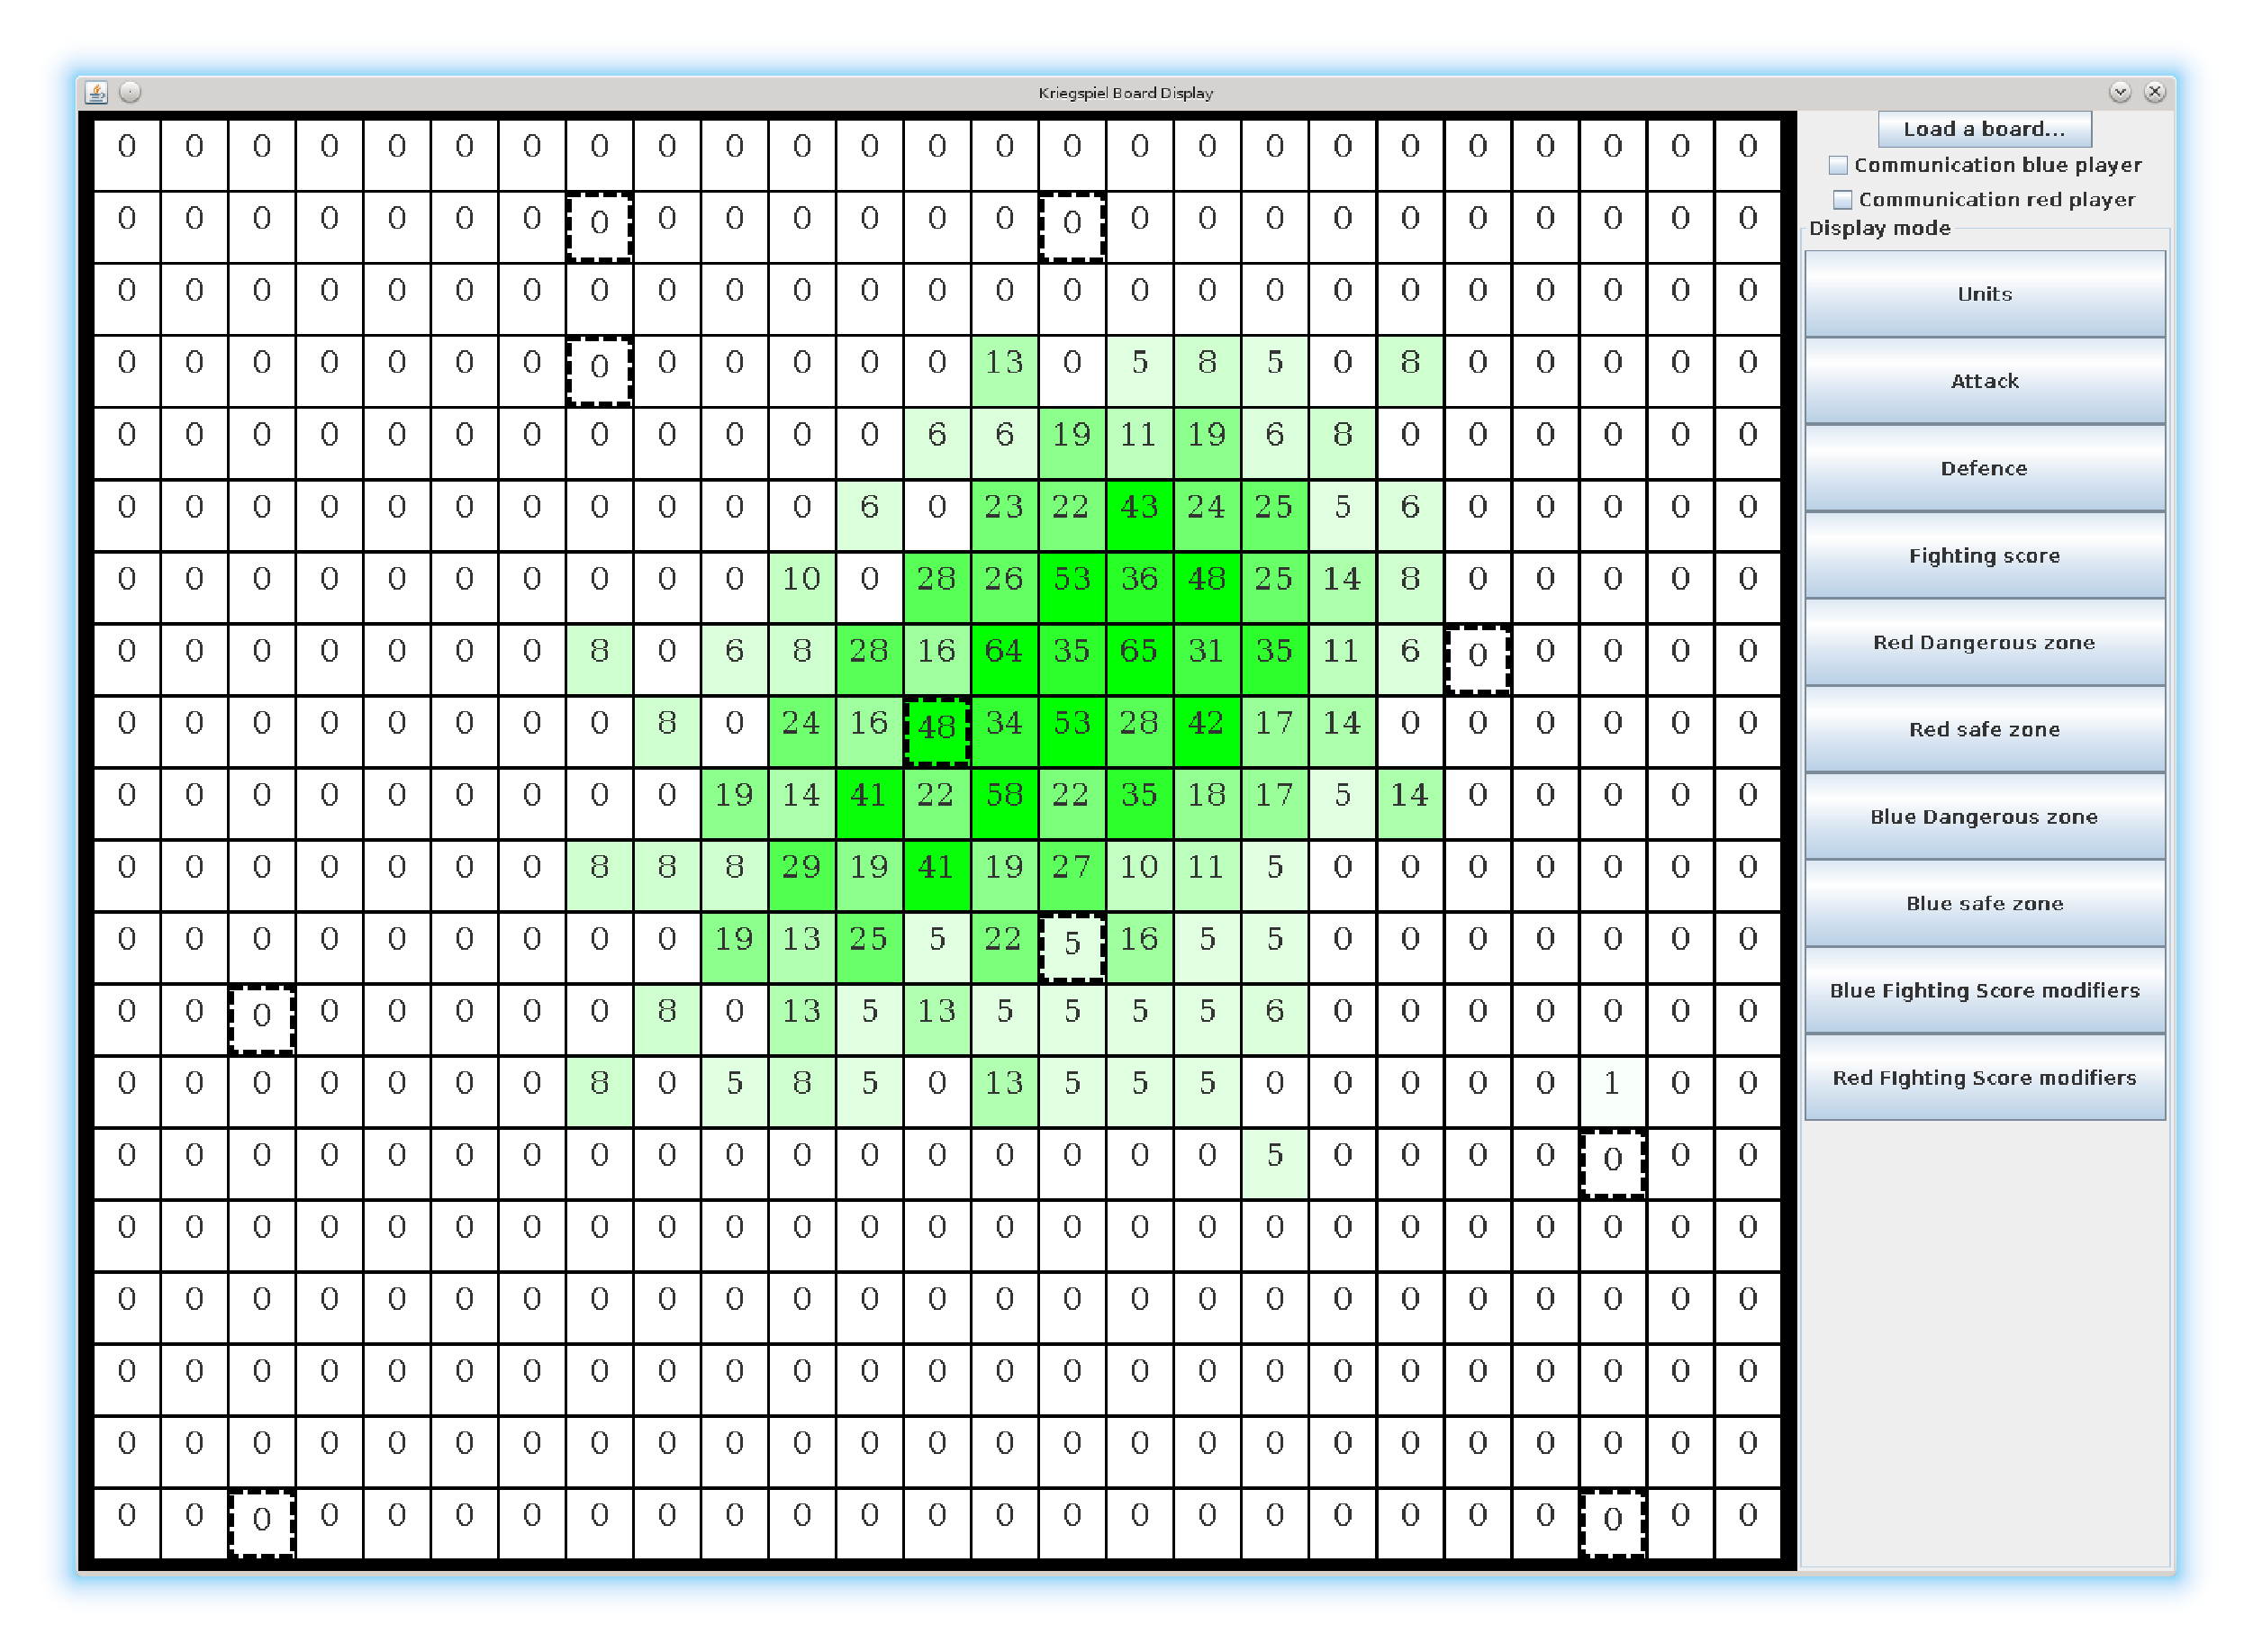
\includegraphics[scale=0.5]{images/screen_safe.eps}}
			Dans les modes zone sûre, la matrice de défense de l'équipe choisie est affichée.
			Dans les modes zone dangereuse, la matrice d'attaque de l'équipe choisie est affichée
			Plus les cases sont foncées, plus elles sont sûres (respectivement dangereuses) pour l'équipe.
			Ici c'est la zone sûre de l'équipe rouge qui est affichée.

			\clearpage

		\subsection{Modes modificateur de score de combat}
			\centerline{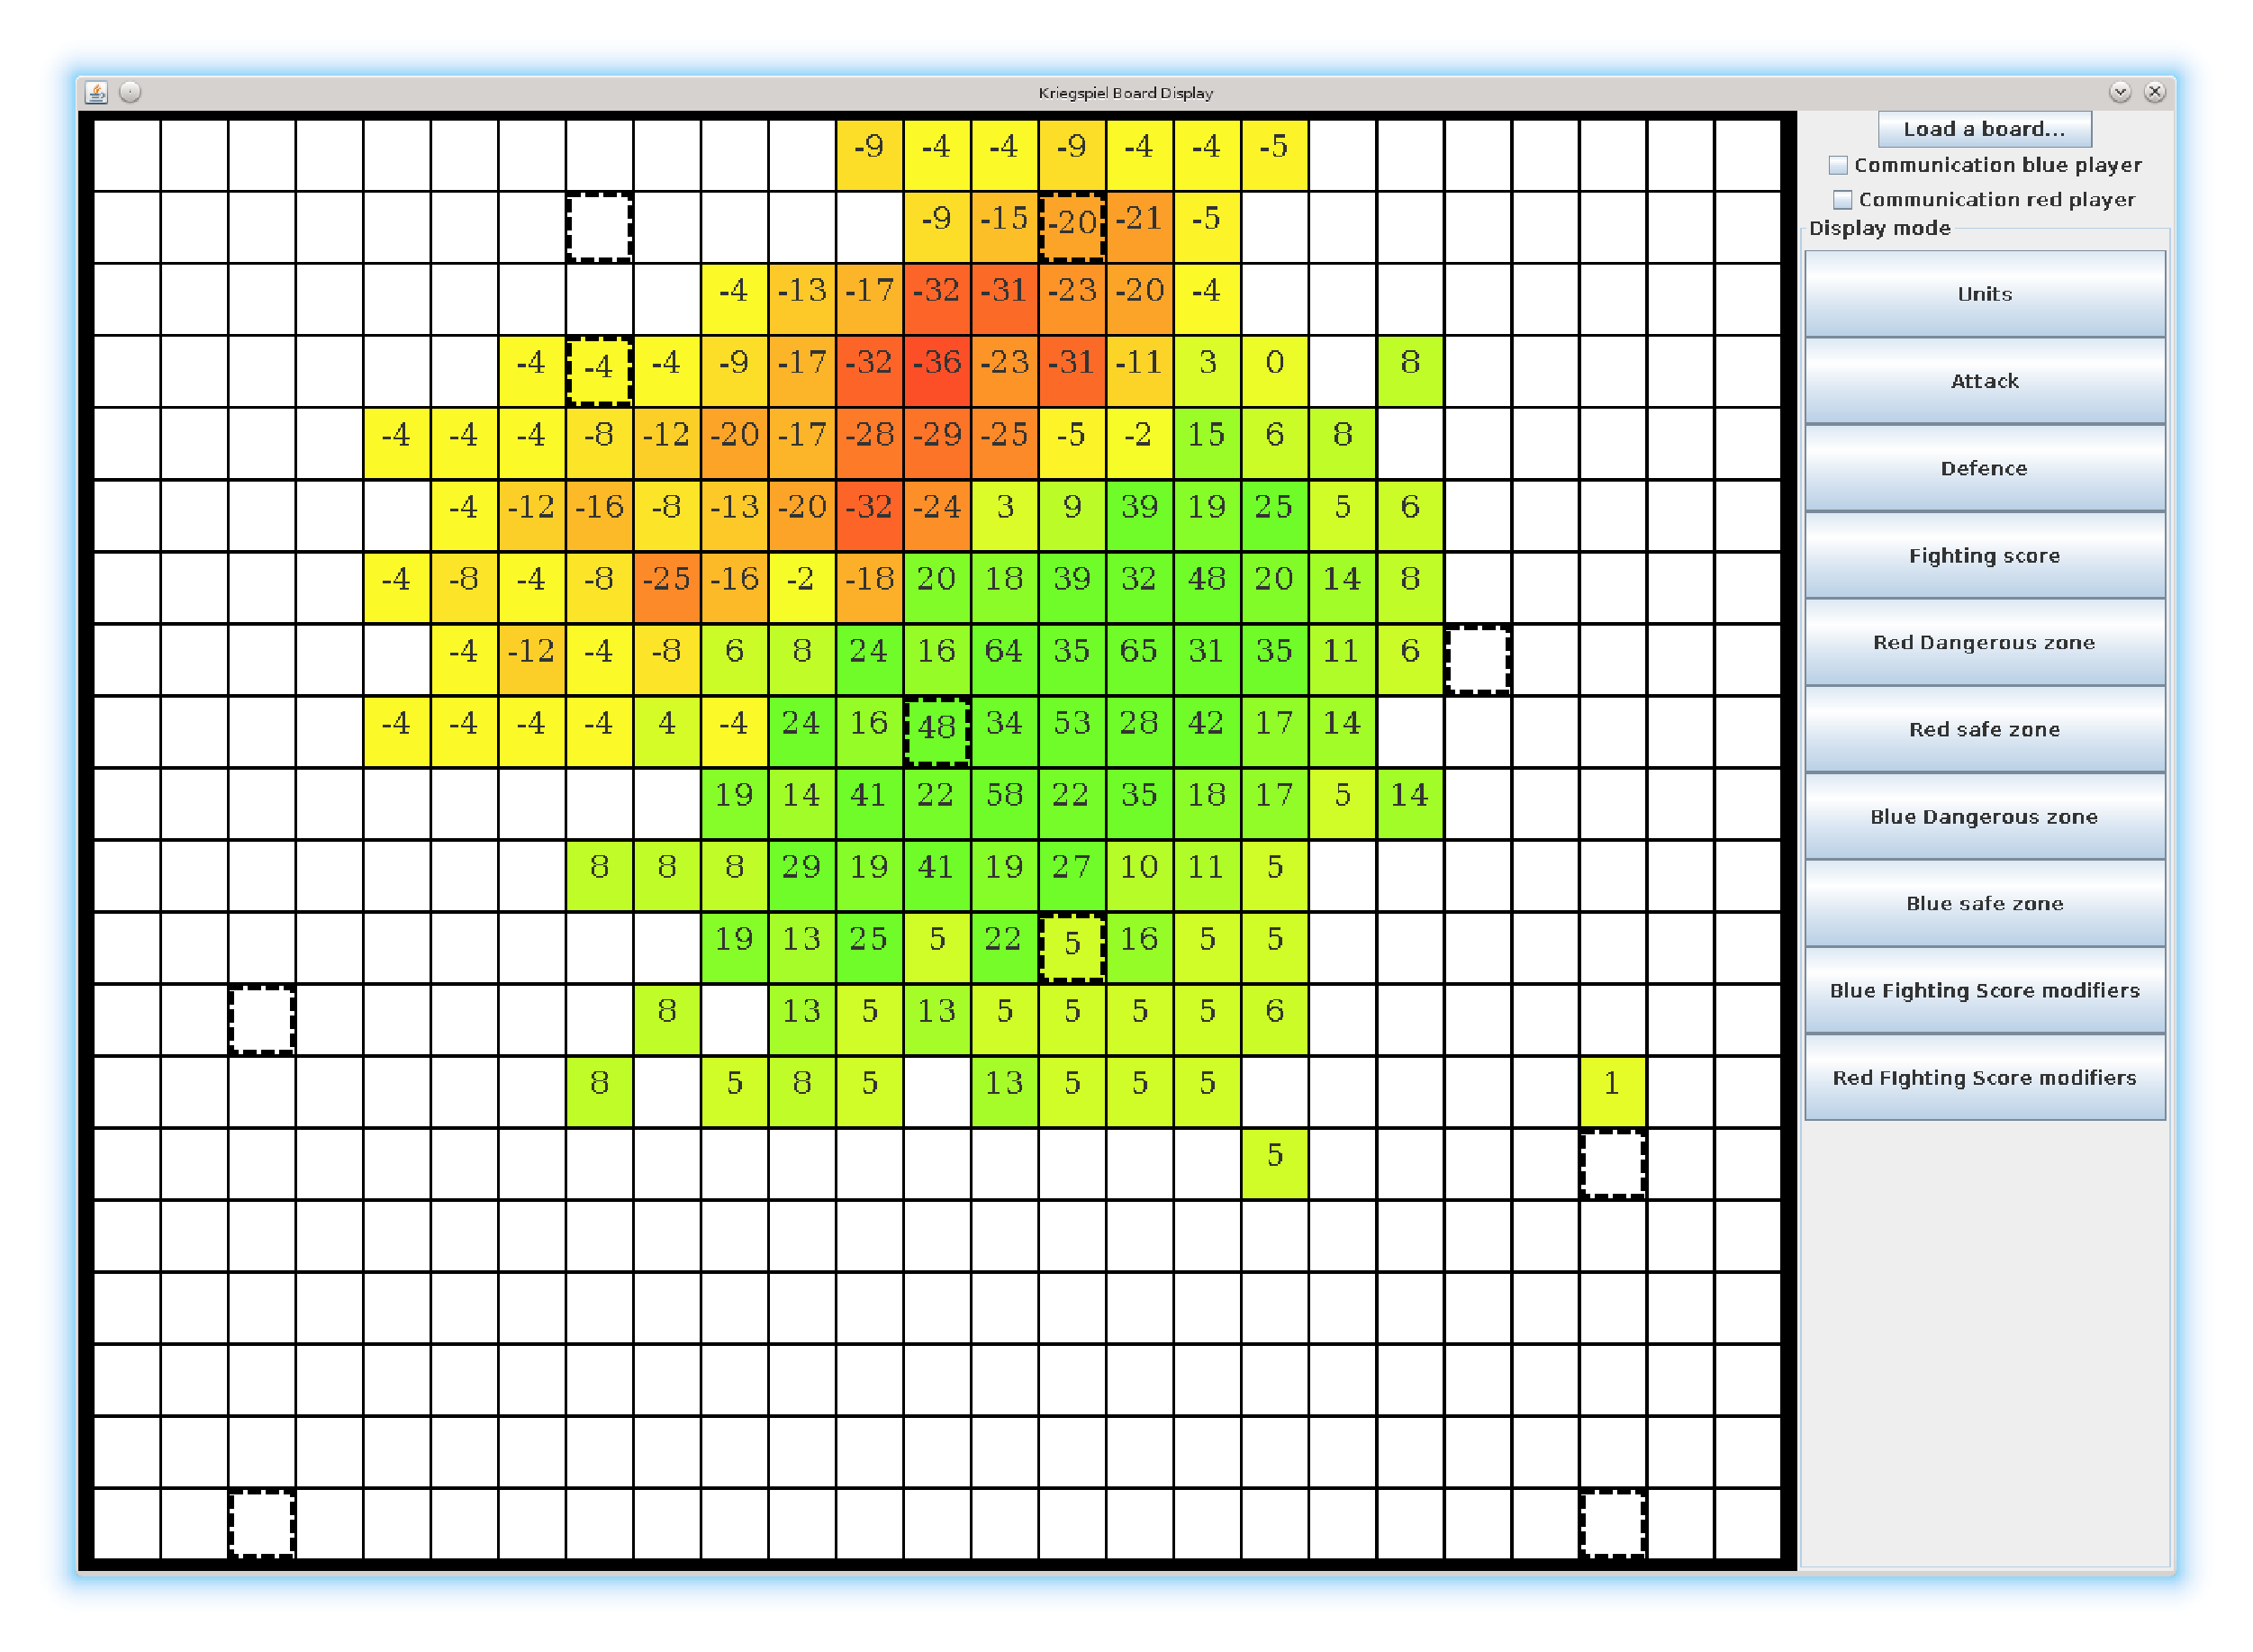
\includegraphics[scale=0.5]{images/screen_fsmod.eps}}
			Dans ces derniers modes d'affichage, on utilise les zones sûres et dangereuses pour calculer pour chaque cas le modificateur
			qui serait appliqué au score de combat d'une unité si elle y était présente.

	\section{Autres fonctionnalités}

		\subsection{Lignes de communication}

			\centerline{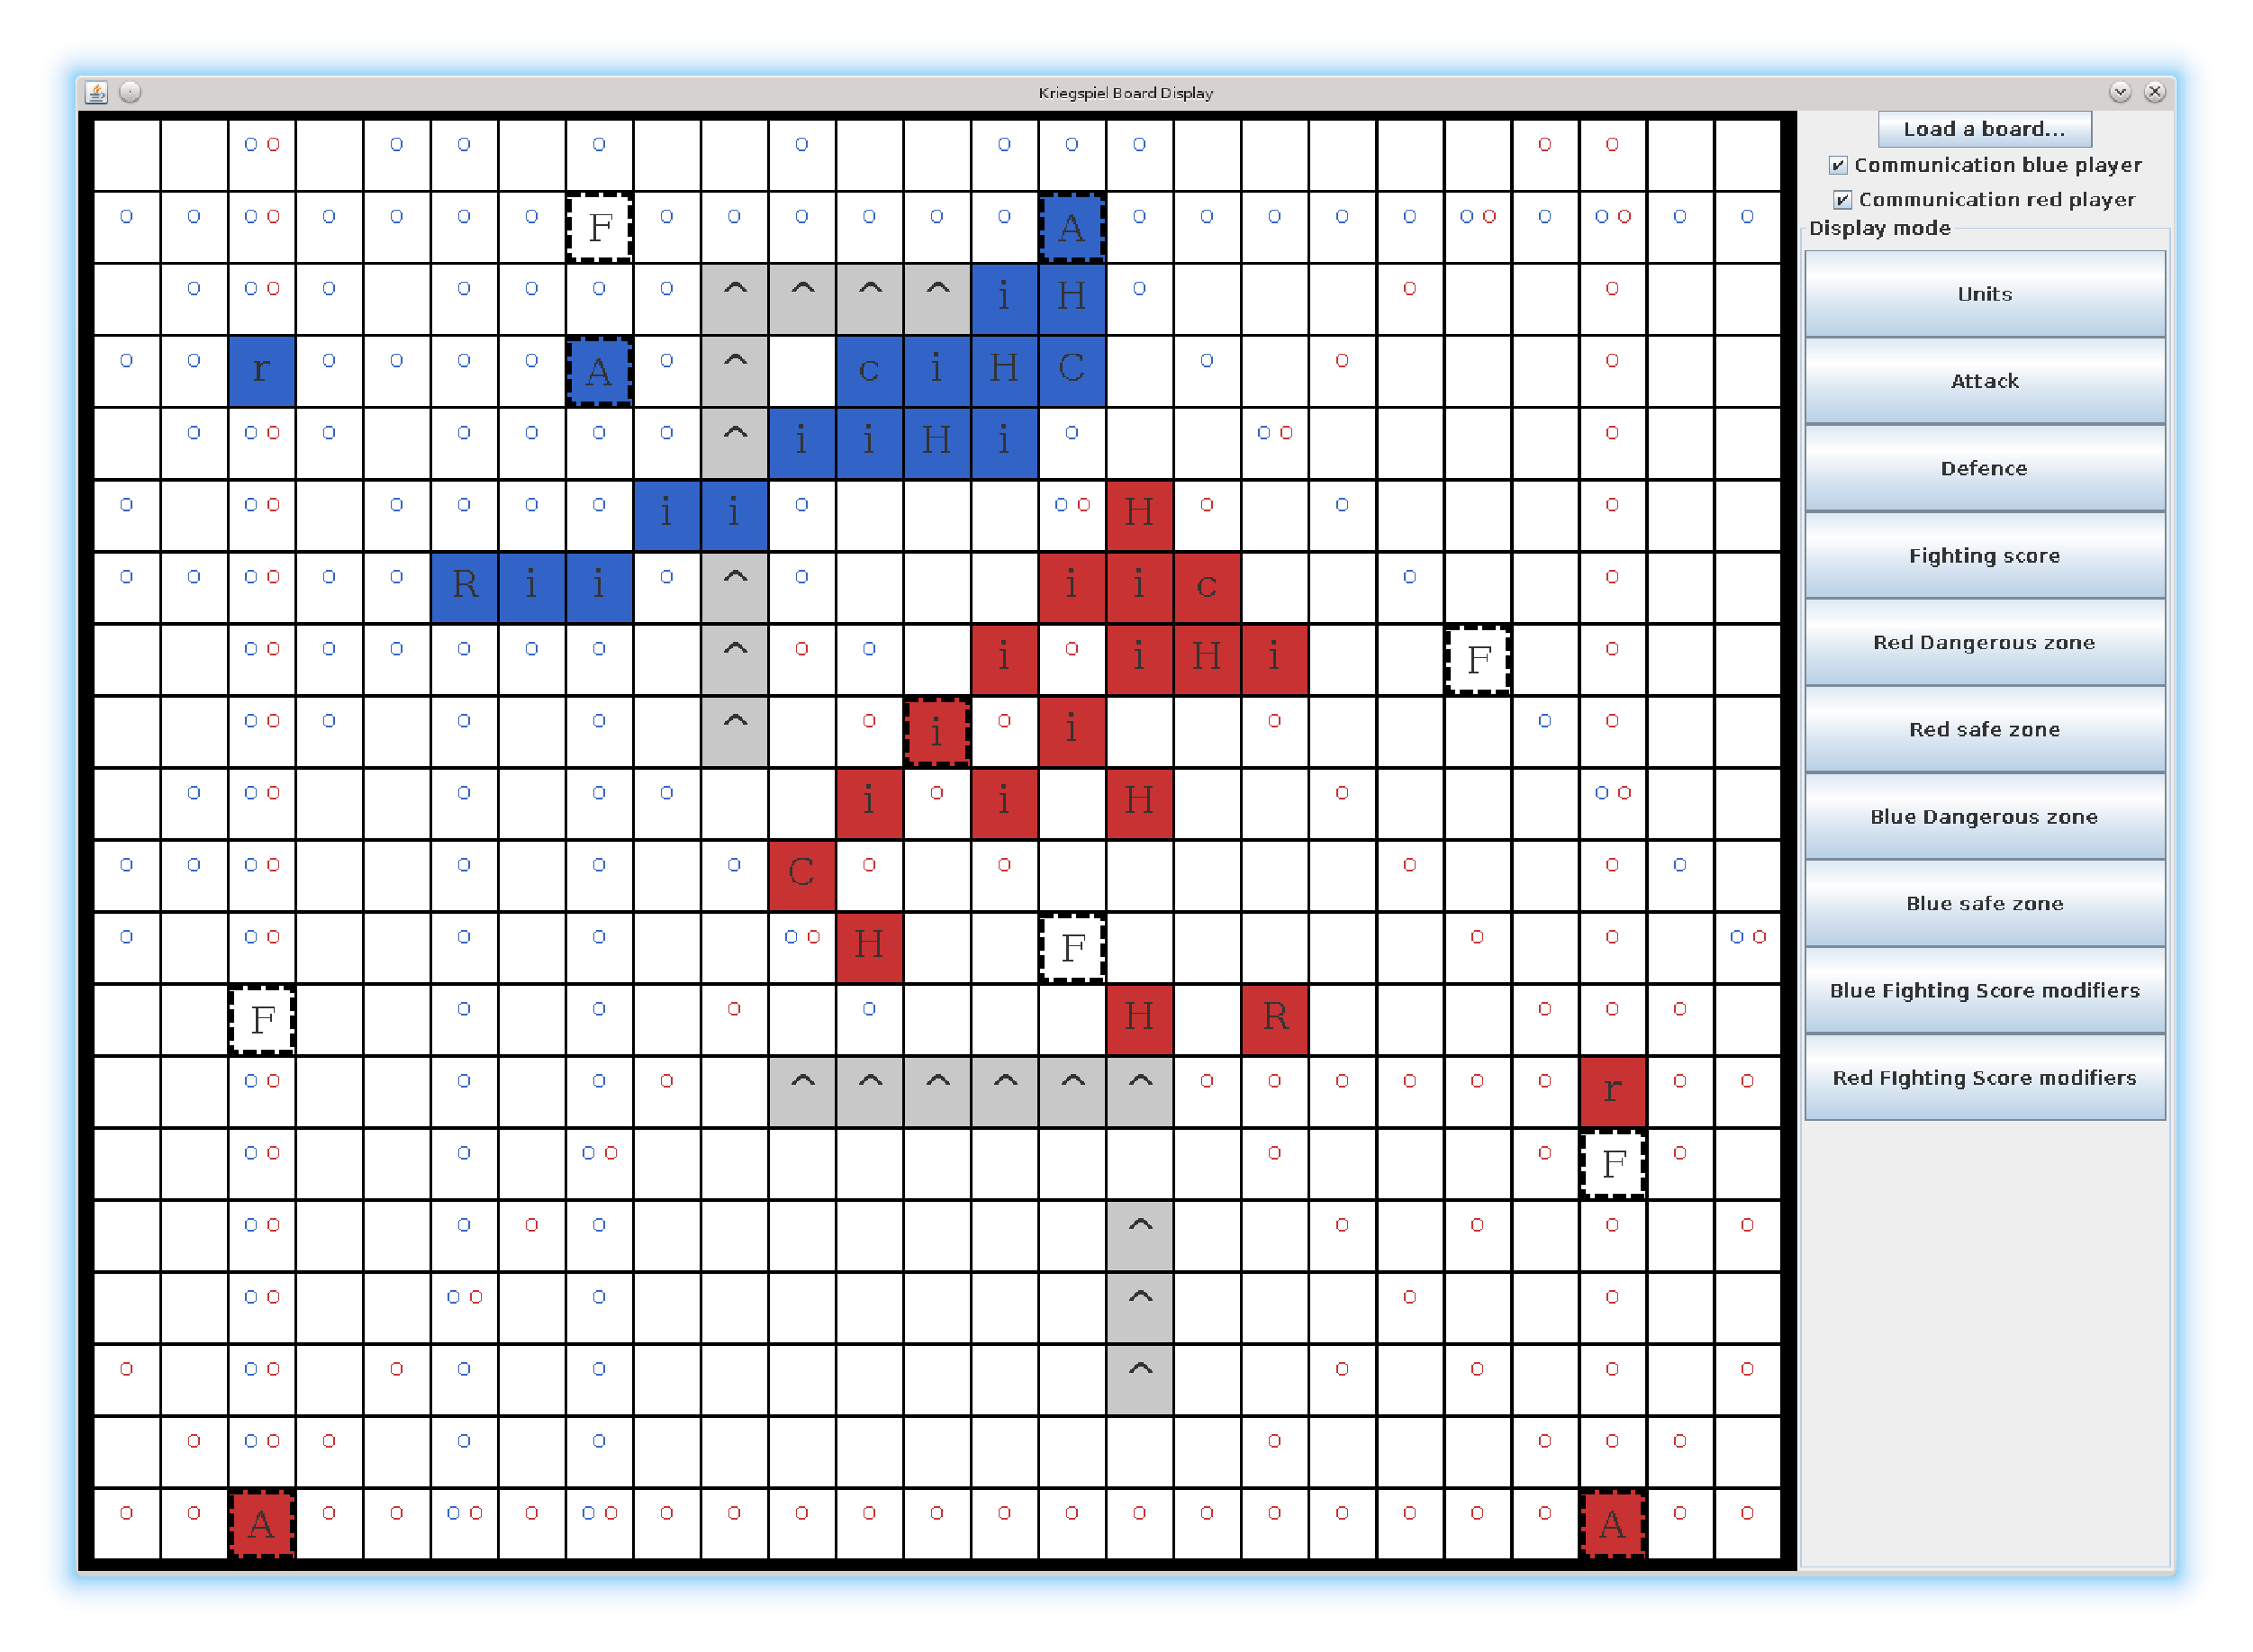
\includegraphics[scale=0.45]{images/screen_com.eps}}
			Les lignes de communication sont représentées par des cercles de la couleur de l'équipe sur les cases vides.
			Les unités déconnectées ont une teinte plus claire que les unités connectées.
			On peut remarquer que les unités adverses bloquent les communications et que les relais alliés les propagent.

			\clearpage

		\subsection{Raccourcis clavier}
			Avant d'implémenter le menu, nous avions mis en place des racourcis clavier afin de modifier rapidement les options d'affichage.
			Ces raccourcis ont été maintenus et fonctionnent correctement de concert avec les boutons mais nous avons cessé d'en rajouter 
			en considérant qu'il était inutile d'apprendre des raccourcis alors qu'un clic sur un bouton est aussi rapide et efficace.
			Il est donc possible d'afficher / cacher les lignes de communications avec les touches 0 et 1 (pour les équipes 0 et 1) du pavé numérique.
			Il est également possible de changer de mode d'affichage entre Unités (u) Attaque (a) et Défense (d)
